\chapter{\IfLanguageName{dutch}{Stand van zaken}{State of the art}} \label{chap:State of the art}%
\label{ch:stand-van-zaken}

% Tip: Begin elk hoofdstuk met een paragraaf inleiding die beschrijft hoe
% dit hoofdstuk past binnen het geheel van de bachelorproef. Geef in het
% bijzonder aan wat de link is met het vorige en volgende hoofdstuk.

% Pas na deze inleidende paragraaf komt de eerste sectiehoofding.

Zoals vermeld in de inleiding heeft het 360°-Zorglab van Hogeschool Gent verschillende doeleinden. Zo kunnen studenten geneeskunde leren hoe ze een operatie moeten uitvoeren zonder iemand als testpersoon te gebruiken. Anderzijds kan het een persoon die plankenkoorts heeft een presentatie of een toespraak leren houden. In deze situatie zal een patiënt met een stotter leren een vlot gesprek te houden wanneer hij bijvoorbeeld op sollicitatie gaat. Dit wordt gerealiseerd aan de hand van 360° opnames die voor de patiënt opnieuw afgespeeld kunnen worden in VR.

\section{\IfLanguageName{dutch}{Stotteren}{Stutter}}%
Stotteren is een spraakstoornis die gekenmerkt wordt door onderbrekingen en verstoringen in het vloeiend spreken. De aandoening komt vaker voor bij kinderen en gaat bij 80\% over naarmate ze opgroeien \autocite{Gordon2002}. Er zijn verschillende types van onvloeiendheid in spraak \autocite{Chee2009}: tussenwerpsels (woorden zoals 'uh' of 'eh'), herzieningen (het aanpassen van de inhoud of de grammaticale structuur van de zin), onafgemaakte zinnen, herhaling, aanhoudende geluiden en afgebroken woorden. Een stotter kan voorkomen in verschillende mate, sommigen zullen meer last hebben zichzelf te uiten terwijl bij anderen de stoornis niet hard opvalt.

De specifieke oorzaak van een stotter is nog niet doorgrond. Uit het onderzoek van \textcite{Gordon2002} blijkt echter dat de rechter- en linkerhersenhelft verschillende en tegenovergestelde rollen lijken te spelen bij het ontstaan van stotteren. Symptomen van stotteren worden geassocieerd met activering van de voorste gebieden in de linkerhersenhelft, terwijl zowel voorste als achterste perisylvische gebieden in de rechterhersenhelft geactiveerd worden wanneer het spreken vloeiender wordt. Deze verbetering kan mogelijk te wijten zijn aan de koppeling van motorische en zintuiglijke gebieden in de rechterhersenhelft.

\section{\IfLanguageName{dutch}{Virtuele realiteit}{Virtual reality}}%
Hoewel Virtual Reality tegenwoordig ver gevorderd is, bestaat het al voor een lange tijd. Het eerste toestel dat de werkelijkheid nabootste was Morton Heilig’s Sensorama\footnote{\href{https://www.historyofinformation.com/detail.php?id=2785}{https://www.historyofinformation.com/detail.php?id=2785}} (Figuur \ref{fig:Sensorama}) uit 1962. Dit liet de gebruiker ervaren hoe het voelde om op een motor door Boston te rijden. In de jaren nadien werden ook andere toestellen uitgevonden zoals de 'Sword of Damocles'\footnote{\href{https://www.dsource.in/course/virtual-reality-introduction/evolution-vr/sword-damocles-head-mounted-display}{https://www.dsource.in/course/virtual-reality-introduction/evolution-vr/sword-damocles-head-mounted-display}} (Figuur \ref{fig:SwordOfDamocles}) die de locatie van het hoofd en de ogen volgde en Nintendo's 'power glove'\footnote{\href{https://en.wikipedia.org/wiki/Power_Glove}{https://en.wikipedia.org/wiki/Power\_Glove}} voor de NES \autocite{Boas2012}.

\begin{figure}
    \begin{subfigure}{.5\textwidth}
        \centering
        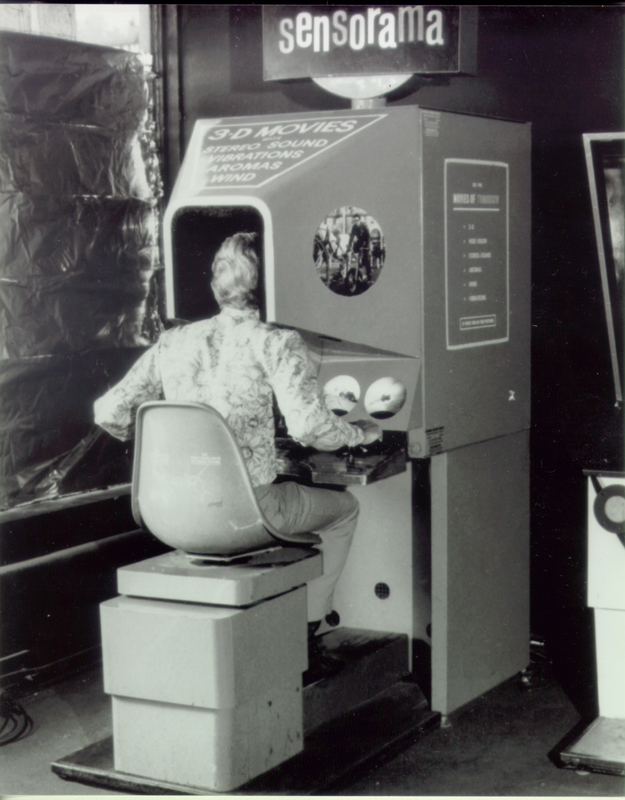
\includegraphics[width=.8\linewidth]{Sensorama.jpg}
        \caption{The Sensorama machine}
        \caption*{Source: \href{https://www.historyofinformation.com/detail.php?id=2785}{https://www.historyofinformation.com/detail.php?id=2785}}
        \label{fig:Sensorama}
    \end{subfigure}%
    \begin{subfigure}{.5\textwidth}
        \centering
        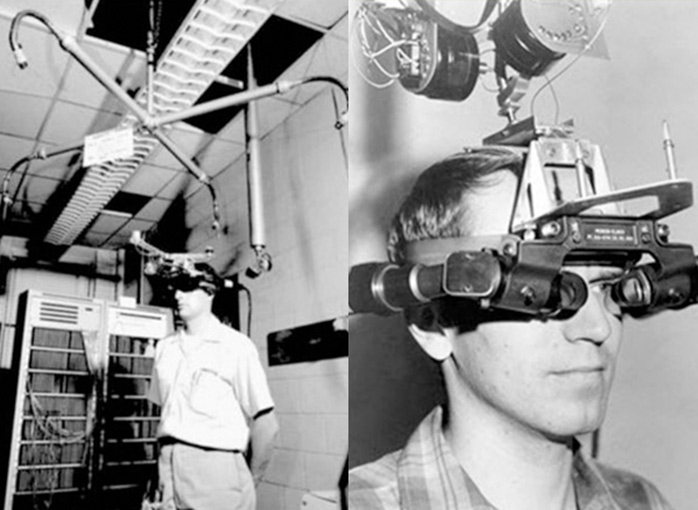
\includegraphics[width=.8\linewidth]{SwordOfDamocles.jpg}
        \caption{Ivan Sutherland's first VR Head Mounted Display, The Sword of Damocles}
        \caption*{Source: \href{https://www.dsource.in/course/virtual-reality-introduction/evolution-vr/sword-damocles-head-mounted-display}{https://www.dsource.in/course/virtual-reality-introduction/evolution-vr/sword-damocles-head-mounted-display}}
        \label{fig:SwordOfDamocles}
    \end{subfigure}
\end{figure}

De eerste vermelding van de term VR daarentegen kwam pas rond 1985 zegt \textcite{Bryson2013}. Hij verteld over hoe Jaron Lanier de term 'virtual reality' gebruikte om het Virtual Interactive Environment Workstation (VIEW) lab van NASA te beschrijven. De daaropvolgende jaren werd de term steeds populairder met tot gevolg dat het ruim werd toegepast op verschillende toepassingen. Daarom moest de term VR goed gedefinieerd worden:

\begin{quote}
    Virtual Reality is the use of computer technology to create the effect of an
    interactive three-dimensional world in which the objects have a sense of spatial
    presence. \autocite{Bryson2013}
\end{quote}

Tegenwoordig zijn VR-toestellen te vinden in vele soorten een maten. Zo zijn er headsets gemaakt voor PC of consoles en anderen voor smartphones. Dankzij software- en hardwareverbeteringen bestaan er nu zelfs headsets die autonoom werken. Dit zorgt ervoor dat kabels en complexe set-ups niet nodig zijn. Deze verbeteringen zorgen ook dat de digitale wereld realistischer aanvoelt.

\section{\IfLanguageName{dutch}{Artificiële intelligentie}{Artificial intelligence}}%
Het afgelopen jaar is de populariteit van AI enorm gestegen, zoals text-to-image models zoals DALL-E 2, Imagen en Stable diffusion die een gegeven tekst prompt kunnen omzetten in afbeeldingen. Daarnaast zijn er ook applicaties die language models gebruiken zoals Chat-GPT, spraak assistenten en Github Copilot. Zij kunnen teksten verwerken en accurate antwoorden genereren op basis van hun kennis ook al zijn deze niet altijd accuraat (Meer hierover in \ref{ssec:Natural Language Classifier})

Om het overschakelen naar een volgend fragment te laten gebeuren zonder begeleiding en zonder veel tijd te verliezen, zouden verbale antwoorden gegeven kunnen worden. Een mooi voorbeeld van een gelijkaardige interactie is het project 'Dimensions in Testimony' van de \textcite{USCShoahFoundation2020}. Daar kunnen bezoekers vragen stellen aan een overlevende van de Holocaust die op voorhand een volledig interview heeft afgelegd. Dit werd mogelijk gemaakt dankzij het systeem dat erachter zit (Figuur \ref{fig:DiTArchitecture}). Dit systeem is opgebouwd uit volgende componenten: een software voor spraakherkenning (ASR) die de gebruikers verbale vraag in tekst omzet, een Natural Language Classifier (NLC) die op basis van de gegenereerde tekst een antwoord via een audio/video fragment voorziet en een mediaspeler die de fragmenten kan afspelen met tussendoor een inactieve animatie \autocite{Traum2015}.

\begin{figure}[h]
    \centering
    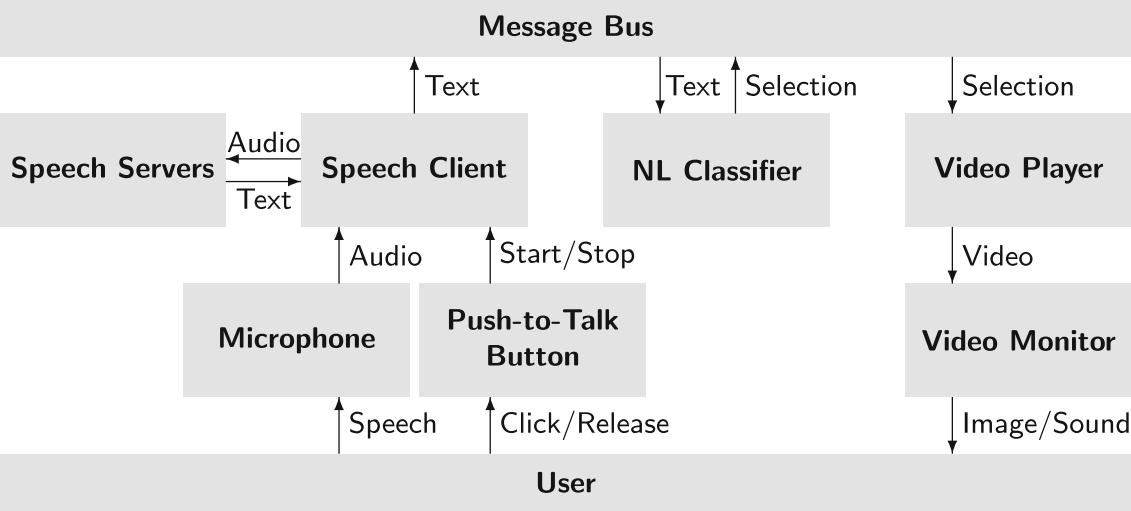
\includegraphics[width=\linewidth*3/4]{TraumDEtAl_DimensionsInTestimony_SystemArchitecture.png}
    \caption{Dimensions in Testimony - Systeem Architectuur \autocite{Traum2015}}
    \label{fig:DiTArchitecture}
\end{figure}

Een ander voorbeeld zijn de home assistenten zoals Google Home, Amazon Echo of Apple HomePod. Zij staan op stand-by tot de gebruiker het triggerwoord zegt, `Hey Google' bijvoorbeeld. Eenmaal geactiveerd luisteren ze naar wat de gebruiker zegt en zetten ze dit aan de hand van een ASR om naar tekst. Daarna haalt het met natuurlijke taalverwerking (NLP) de intentie en sleutelwoorden uit de tekst en genereert daarmee een gepast antwoord. Als laatste zet het gegenereerde tekst om naar spraak.

\subsection{\IfLanguageName{dutch}{Spraakherkening}{Speech recognition}}%

Net als VR is spraakherkenning de laatste jaren veel vooruitgegaan, dit komt omdat er meer data beschikbaar is, de computers sneller en de algoritmes, genaamd deep neural networks, beter zijn \autocite{Hessen2020}. Deze netwerken worden getraind op grote datasets bestaande uit diverse spraakfragmenten. Hieruit leert het de patronen en kenmerken van menselijke spraak. Maar perfect zullen ze nooit zijn zegt \textcite{Hessen2020}. Dit is geen verrassing aangezien mensen zelf nog vaak problemen hebben bij het verstaan van een andere. Er zijn verschillende stappen waar de ASR de fout kan ingaan.

\paragraph{\IfLanguageName{dutch}{Domeinproblemen}{Domain problems}}%
Onder de domein problemen valt ten eerste galm en geluidshinder. Dit komt voor wanneer een opname gemaakt wordt in een omgeving met veel achtergrond lawaai. Net als mensen heeft de ASR moeilijkheden met het verstaan van de spreker wanneer deze overstemd wordt door de omgeving \autocite{Alharbi2021}. Er zijn verschillende manieren om dit probleem te beperken. Zo wordt het aangeraden om het fragment op te nemen in een rustige omgeving. Als het audiobestand toch veel geruis of achtergrondlawaai bevat is het ook mogelijk dit bestand door een stem extractie software te halen zoals Vocal Remover\footnote{\href{https://vocalremover.org/nl/}{https://vocalremover.org/nl/}}. Het originele doel van deze tool is om de zang van de instrumenten te scheiden in een lied maar dit werkt ook voor gewone spraakbestanden. Naast galm en geluidshinder is het ook moeilijker wanneer twee of meer mensen door elkaar spreken. Dit heet spraak overlapping. Hoe meer mensen in hetzelfde geluidsfragment door elkaar spreken hoe moeilijker het wordt om de spraak te herkennen. Daarom raad \textcite{Hessen2020} aan om een microfoon per spreker aan te brengen. Dit zorgt ervoor dat er voor elke spreker een ander geluidsfragment beschikbaar is om te transcriberen. Een derde domein probleem is domain mismatch. Dit houdt in dat er een discrepantie is tussen het domein gebruikt voor het model te trainen en de use case waar het model in wordt gebruikt. Zo zijn bijvoorbeeld nieuwe accenten of andere omgevingen onbekend voor het model. Daarnaast kan het doeleinde een ander jargon bevatten wat leidt tot out-of-vocabulary fouten.\autocite{Alharbi2021}

\paragraph{\IfLanguageName{dutch}{Natuurlijke taalverwerking}{Natural language processing}}%
Zoals vermeld in de vorige paragraaf is de use case van groot belang. De taal die gebruikt wordt verschilt op vele manieren: jongeren gebruiken andere woorden dan hun senioren, iemand in de IT sector heeft een andere woordenschat dan een dokter. Deze verschillen kunnen leiden tot out-of-vocabulary fouten. Dit houd in dat een bepaald model niet getraind is op bepaalde manier van spreken of woordenschat. Een andere oorzaak van OOV is het trainen van een model op een te kleine dataset. \autocite{Alharbi2021}

Ook niet iedereen spreekt woorden op dezelfde manier uit. Afhankelijk van de sprekers afkomst zullen ze een bepaalde taal met een bepaald dialect spreken. Ook wanneer ze in een taal anders dan hun moedertaal praten zal er vaak sporen van hun eigen taal herkenbaar blijven. Dit zorgt ervoor dat de uitspraak van een woord niet altijd hetzelfde is. \autocite{Alharbi2021}

\paragraph{\IfLanguageName{dutch}{Efficiëntie van apparatuur}{Device efficiency}}%
Als laatste hebben we de gebruikte toestellen. De kwaliteit van de opnameapparatuur kan de nauwkeurigheid van de ASR beïnvloeden. Het gebruikmaken van een high-end microfoon tegenover een goedkope kan betere resultaten creëren. \autocite{Alharbi2021}


\paragraph{\IfLanguageName{dutch}{Sotteren}{Stuttering}}%
De moeilijkheden waarmee een ASR te maken krijgt bij stotter zijn als volgt: herhaling, verlengingen en blokkeringen \autocite{Manjula2019}. In het onderzoek van \textcite{Suryaa2017} bespreken ze verschillende manieren om stotterfragmenten te transcriberen. Zo kan er een model getraind worden op vele stotterfragmenten om zo beter met stottermomenten om te gaan. Een andere aanpak is om vooraf de stottermomenten uit het audiofragment manueel of met andere software te verwijderen. Dat verwerkte fragment wordt daarna pas naar de ASR verstuurd.


\subsection{\IfLanguageName{dutch}{Begrijpen van natuurlijke taal}{Natural Language Understanding}} \label{ssec:Natural Language Classifier}%

Naast de ASR hebben we ook het begrijpen van natuurlijke taal (NLU). In 'Dimension in Testimony' maakten ze hiervoor gebruik van NCPEditor (Figuur \ref{fig:NPCEArchitecture}). De classifier in dit systeem berekent welke antwoorden op de ingegeven tekst kunnen gegeven worden door de taalmodellen van beide te vergelijken en de antwoorden te rangschikken. Zolang de ingegeven tekst een foutmarge lager dan 50\% blijft, zal het antwoord ongewijzigd blijven \autocite{Leuski2010}.

Een andere bekend taalmodel is GPT-3. Dit model ligt aan de basis van de populaire chatbot ChatGPT.

\begin{figure}[h]
    \centering
    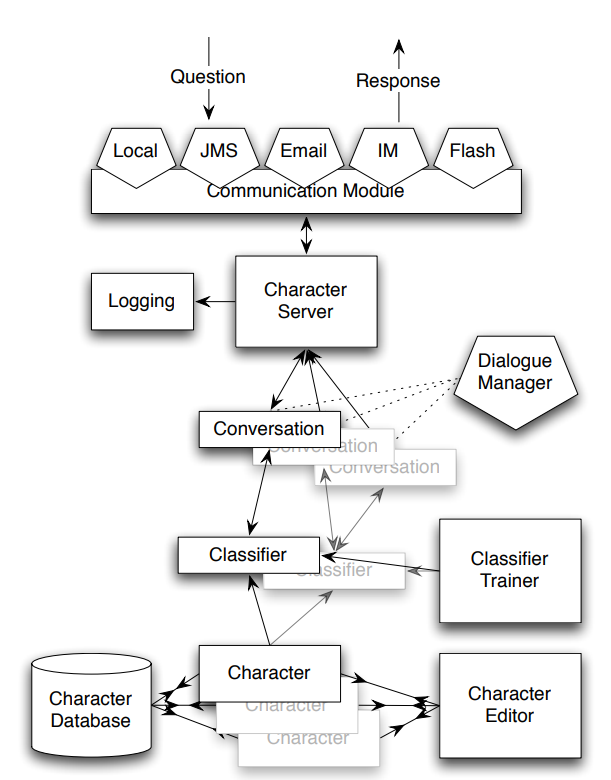
\includegraphics[width=\linewidth*3/4]{Traum&Leuski_NPCEditor_System architecture.png}
    \caption{NPCEditor - Systeem Architectuur \autocite{Leuski2010}}
    \label{fig:NPCEArchitecture}
\end{figure}

\section{\IfLanguageName{dutch}{Long list spraakherkening}{Long list speech recognition}}\label{sec:Speech recognition}%

\subsection{Google Cloud Speech-to-text API}%

\paragraph{\IfLanguageName{dutch}{Beschrijving}{Description}}
Google Cloud Speech-to-text API\footnote{\href{https://cloud.google.com/speech-to-text}{https://cloud.google.com/speech-to-text}} is Google's kijk op spraakherkennigssoftware. De API is heel betrouwbaar. Zo heeft het volgens \textcite{Anggraini2018} een succespercentage van 100\% voor normale Engelse stemmen en een percentage tussen 83,3\% en 90\% voor mensen met een spraakbeperking. Daarnaast biedt het ook de mogelijkheid om het model uit te breiden door het nieuwe vocabulaire aan te leren.

\paragraph{\IfLanguageName{dutch}{Functies}{Features}}
De service komt met verschillende functies. Dit zijn de belangrijke kenmerken die ze adverteren:

\begin{itemize}
    \item \textbf{Taalherkenning}: De API ondersteunt spraakherkenning in verschillende talen en dialecten, waardoor gebruikers wereldwijd toegang hebben tot de dienst. Het kan automatisch de gesproken taal detecteren zonder voorafgaande taalconfiguratie.

    \item \textbf{Real-time streaming}: De API ondersteunt real-time streaming van spraak naar tekst, waardoor ontwikkelaars toepassingen kunnen bouwen die directe feedback en interactie vereisen, zoals live ondertiteling, spraakgestuurde commando's en real-time transcriberen.

    \item \textbf{Hoge nauwkeurigheid}: Dankzij de geavanceerde neurale netwerkmodellen levert de Speech-to-Text API nauwkeurige transcripties, zelfs in omgevingen met achtergrondgeluiden, verschillende spreekstijlen en spraak van meerdere sprekers.

    \item \textbf{Aanpasbare modellen}: Gebruikers kunnen de spraakherkenning aanpassen aan specifieke woordenschat en domeinen door aangepaste woordenlijsten en grammatica's te gebruiken. Dit verhoogt de nauwkeurigheid en zorgt voor een betere herkenning van vakspecifieke terminologie.

    \item \textbf{Multimediaondersteuning}: De API kan spraak herkennen in verschillende formaten, waaronder audio-opnamen, audiobestanden en streaming-audio. Dit maakt integratie met verschillende bronnen en toepassingen mogelijk.

    \item \textbf{Beveiliging en privacy}: Google Cloud hanteert strenge beveiligingsmaatregelen om de vertrouwelijkheid en integriteit van de gegevens te waarborgen. De API ondersteunt ook automatische verwijdering van persoonlijk identificeerbare informatie (PII) uit de gegenereerde transcripties.

    \item \textbf{Spraakherkenning op apparaat}: Naast de cloudgebaseerde API biedt Google Cloud ook een on-device spraakherkenning SDK aan, genaamd Speech-to-Text On-Device. Hiermee kunnen ontwikkelaars spraakherkenning rechtstreeks op apparaten uitvoeren, zonder een internetverbinding te vereisen.
\end{itemize}

\paragraph{\IfLanguageName{dutch}{Tarieven}{Pricing}}
De service kan per maand 60 minuten gratis gebruikt worden. Daarna moet er betaald worden per minuut van €0,016 voor standaard met datalogging tot €0,072 voor medisch gebruik zonder datalogging.

\subsection{Amazon Transcribe}%

\paragraph{\IfLanguageName{dutch}{Beschrijving}{Description}}
Amazon Web Services (AWS) biedt een ASR software aan genaamd Amazon Transcribe\footnote{\href{https://aws.amazon.com/transcribe/}{https://aws.amazon.com/transcribe/}}.

\paragraph{\IfLanguageName{dutch}{Functies}{Features}}
De functies die Amazon Transcribe aanbiedt zijn:

\begin{itemize}
    \item \textbf{Taalherkenning}: Amazon Transcribe kan automatisch de gesproken taal detecteren, waardoor het mogelijk is om meertalige spraakherkenning te realiseren zonder voorafgaande taalconfiguratie.

    \item \textbf{Real-time streaming}: Amazon Transcribe heeft real-time streaming van spraak naar tekst, wat ideaal is voor toepassingen zoals live ondertiteling, spraakgestuurde opdrachten en interactieve dialoogsystemen.

    \item \textbf{Overzichtelijke transcripties}: Dit wordt gedaan door het toevoegen van tijdsaanduidingen en het herkennen van meerdere stemmen.

    \item \textbf{Aanpassing van modellen}: Gebruikers kunnen de spraakherkenning verbeteren en aanpassen aan specifieke vocabulaires en domeinen door aangepaste taalmodellen te maken. Hierdoor kunnen ze de nauwkeurigheid van de herkenning verhogen voor gespecialiseerde toepassingen.

    \item \textbf{Privacy}: Amazon Transcribe garandeert beveiligde dataverkeer. Daarnaast is het ook mogelijk woorden uit de transcriptie te filteren als deze ongewenst zijn.
\end{itemize}

\paragraph{\IfLanguageName{dutch}{Tarieven}{Pricing}}
De service kan 60 minuten per maand gratis gebruikt worden, gedurende 12 maanden. Daarna moet er een vergoeding worden betaald afhankelijk van het totale gebruik per maand en de geolocatie van de gebruikte server (Figuur \ref{fig:PricingAmazonTranscribe}).

\begin{figure}[h]
    \centering
    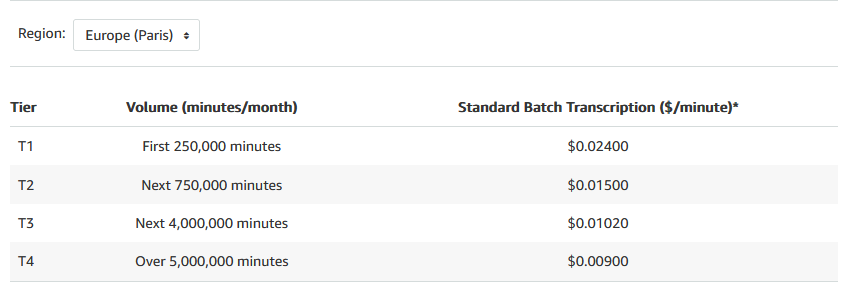
\includegraphics[width=\linewidth*3/4]{graphics/AmazonTranscribePricing.png}
    \caption{Prijzen Amazon Transcribe voor Parijse server \autocite{Amazon2023}}
    \label{fig:PricingAmazonTranscribe}
\end{figure}

\subsection{Microsoft Azure Speech Services}%

\paragraph{\IfLanguageName{dutch}{Beschrijving}{Description}}
Microsoft Azure Speech Services\footnote{\href{https://azure.microsoft.com/en-us/products/ai-services/speech-to-text}{https://azure.microsoft.com/en-us/products/ai-services/speech-to-text}} is een spraakherkenningsservice die wordt aangeboden door Microsoft Azure, het cloudplatform van Microsoft.

\paragraph{\IfLanguageName{dutch}{Functies}{Features}}
Azure Speech Services biedt een breed scala aan functies voor spraakherkenning en tekst-naar-spraak-conversie. Enkele van de belangrijkste functies zijn:

\begin{itemize}
    \item \textbf{Spraakherkenning}: De service kan gesproken taal detecteren en omzetten naar tekst in meer dan 60 talen. Het ondersteunt zowel real-time verwerking als batchverwerking van audiobestanden.

    \item \textbf{Taalherkenning}: Azure Speech Services kan automatisch de gesproken taal detecteren, waardoor het mogelijk is om meertalige spraakherkenning te realiseren zonder voorafgaande taalconfiguratie.

    \item \textbf{Aanpassing van modellen}: Gebruikers kunnen de spraakherkenning verbeteren en aanpassen aan specifieke vocabulaires en domeinen door aangepaste taalmodellen te maken. Hierdoor kunnen ze de nauwkeurigheid van de herkenning verhogen voor gespecialiseerde toepassingen.

    \item \textbf{Real-time streaming}: Azure Speech Services ondersteunt real-time streaming van spraak naar tekst, wat ideaal is voor toepassingen zoals live ondertiteling, spraakgestuurde opdrachten en interactieve dialoogsystemen.

    \item \textbf{Text-to-speech}: Naast spraakherkenning biedt de service ook mogelijkheden voor tekst-naar-spraak-conversie. Gebruikers kunnen tekst invoeren en de service genereert menselijke spraakuitvoer in verschillende stemmen en talen.
\end{itemize}

\paragraph{\IfLanguageName{dutch}{Tarieven}{Pricing}}
Per maand bied Azure vijf uur gratis aan daarna moet er een vergoeding van €0,935 betaald worden per uur.

\subsection{Mozilla DeepSpeech}%

\paragraph{\IfLanguageName{dutch}{Beschrijving}{Description}}
In tegenstelling tot de voorgaande services is DeepSpeech van Mozilla open source.

\paragraph{\IfLanguageName{dutch}{Functies}{Features}}
Mozilla DeepSpeech\footnote{\href{https://deepspeech.readthedocs.io/en/r0.9/}{https://deepspeech.readthedocs.io/en/r0.9/}} biedt verschillende functies en mogelijkheden voor spraakherkenning. Enkele van de belangrijkste kenmerken zijn:

\begin{itemize}
    \item \textbf{Hoge nauwkeurigheid:} DeepSpeech streeft naar hoge nauwkeurigheid in spraakherkenning en heeft aanzienlijke vooruitgang geboekt in termen van herkenningsscores.

    \item \textbf{Flexibiliteit:} Het systeem kan worden aangepast en afgestemd op specifieke toepassingen of vocabulaires. Hierdoor kan het worden gebruikt voor uiteenlopende spraakherkenningsscenario's.

    \item \textbf{Real-time verwerking:} DeepSpeech is ontworpen om spraak in realtime om te zetten, wat betekent dat het geschikt is voor toepassingen die onmiddellijke spraak-naar-tekstfunctionaliteit vereisen.

    \item \textbf{Privacy:} Als open-sourceproject stelt DeepSpeech gebruikers in staat om spraakherkenningssystemen lokaal uit te voeren, waardoor de privacy van gebruikersinformatie beter gewaarborgd is.
\end{itemize}

\paragraph{\IfLanguageName{dutch}{Tarieven}{Pricing}}
Aangezien dat de service open source is, moet er geen vast tarief betaald worden voor de service. Er kunnen echter wel kosten komen om de service te hosten.

\subsection{Whisper}%

\paragraph{\IfLanguageName{dutch}{Beschrijving}{Description}}
Whisper\footnote{\href{https://openai.com/research/whisper}{https://openai.com/research/whisper}} is de ASR service gemaakt door OpenAI. Het is beschikbaar als een API die ontwikkelaars kunnen integreren in hun eigen toepassingen en systemen door er spraakopnamen naar te sturen. De API geeft vervolgens een tekstuele weergave van de spraak terug als respons.

\paragraph{\IfLanguageName{dutch}{Functies}{Features}}
Whisper heeft verschillende kenmerken en mogelijkheden die het tot een krachtig spraakherkenningssysteem maken:

\begin{itemize}
    \item \textbf{Hoge nauwkeurigheid:} Whisper heeft aanzienlijke vooruitgang geboekt in termen van spraakherkenningsscores en streeft naar hoge nauwkeurigheid bij het omzetten van spraak naar tekst.

    \item \textbf{Meertaligheid:} Het model van Whisper ondersteunt meerdere talen, waardoor het geschikt is voor wereldwijde toepassingen en gebruikers met verschillende taalvereisten.

    \item \textbf{Flexibiliteit:} Whisper kan worden aangepast en afgestemd op specifieke toepassingen en vocabulaires, waardoor het kan worden gebruikt in uiteenlopende spraakherkenningsscenario's.

    \item \textbf{Real-time verwerking:} Het systeem is ontworpen om spraak in realtime te verwerken, wat betekent dat het geschikt is voor toepassingen die onmiddellijke spraak-naar-tekstfunctionaliteit vereisen.

    \item \textbf{Privacy:} OpenAI hanteert strenge beveiligings- en privacyrichtlijnen om de gebruikersgegevens te beschermen. Whisper stelt gebruikers in staat om spraakherkenningssystemen lokaal uit te voeren, waardoor de privacy van gebruikersinformatie beter gewaarborgd is.
\end{itemize}

\paragraph{\IfLanguageName{dutch}{Tarieven}{Pricing}}
Net als Mozilla's DeepSpeech is Whisper open source. Dit betekent dat de kosten afhangen van waar en hoe de service wordt gehost.

\subsection{Kaldi ASR}

\paragraph{\IfLanguageName{dutch}{Beschrijving}{Description}}
Kaldi ASR\footnote{\href{https://kaldi-asr.org/}{https://kaldi-asr.org/}} is een open-source spraakherkenningssysteem dat algemeen wordt gebruikt in de academische wereld en de IT industrie. Het is ontwikkeld door het Kaldi-project, een community-gedreven initiatief dat zich richt op het leveren van state-of-the-art spraaktechnologie.

Kaldi maakt gebruik van geavanceerde algoritmen en technieken, waaronder deep neural networks (DNN's) en hidden Markov models (HMM's), om spraak naar tekst om te zetten. Het biedt een flexibel en configureerbaar framework dat kan worden aangepast aan verschillende spraakherkenningstoepassingen.

\paragraph{\IfLanguageName{dutch}{Functies}{Features}}
Kaldi ASR biedt een breed scala aan functies en mogelijkheden die het tot een krachtig spraakherkenningssysteem maken:

\begin{itemize}
    \item \textbf{Hoge nauwkeurigheid:} Kaldi maakt gebruik van geavanceerde modellen en trainingstechnieken om nauwkeurige resultaten te leveren.

    \item \textbf{Flexibiliteit:} Het Kaldi-framework is zeer configureerbaar en aanpasbaar. Het stelt gebruikers in staat om modellen en akoestische kenmerken aan te passen aan specifieke toepassingen en datasets.

    \item \textbf{Meertaligheid:} Kaldi ondersteunt meerdere talen en kan worden gebruikt voor spraakherkenning in verschillende taalomgevingen.

    \item \textbf{Uitgebreide toolkit:} Kaldi wordt geleverd met een uitgebreide toolkit die verschillende hulpmiddelen en utilities biedt voor spraakdataverwerking, modeltraining en evaluatie.

    \item \textbf{Community-ondersteuning:} Het Kaldi-project wordt ondersteund door een actieve gemeenschap van ontwikkelaars en onderzoekers, wat resulteert in regelmatige updates, bugfixes en nieuwe functies.
\end{itemize}

\paragraph{\IfLanguageName{dutch}{Gebruik en implementatie}{Usage and implementation}}
Kaldi ASR wordt meestal gebruikt via de command line-interface en vereist enige technische kennis om effectief te kunnen gebruiken. Het proces om Kaldi te gebruiken omvat het verzamelen en voorbereiden van spraakgegevens, het trainen van akoestische en taalmodellen, en het uitvoeren van de spraakherkenning op nieuwe gegevens.

Kaldi biedt documentatie en handleidingen om gebruikers te begeleiden bij de implementatie en het gebruik van het systeem. Het heeft een actieve gebruikersgemeenschap waar gebruikers vragen kunnen stellen en ervaringen kunnen delen.

\paragraph{\IfLanguageName{dutch}{Beschikbaarheid en prijs}{Availability and pricing}}
Kaldi ASR is een open-source project en is vrij beschikbaar voor iedereen. Het kan worden gedownload van de officiële Kaldi-website en lokaal worden uitgevoerd.


\section{\IfLanguageName{dutch}{Long list natuurlijke taalverwerking}{Long list Natural Language Classifiers}} \label{sec:Natural Language Classifier}%

\subsection{GPT series}%

\paragraph{\IfLanguageName{dutch}{Beschrijving}{Description}}
The GPT-series, wat staat voor Generative Pre-trained Transformer, zijn algemene taalmodellen gemaakt door OpenAI. Het doel van deze modellen is genereren van menselijke taal op basis van de gegeven input. Het meest bekende voorbeeld is OpenAI's chatbot, ChatGPT\footnote{\href{https://openai.com/blog/chatgpt}{https://openai.com/blog/chatgpt}}. Het  maakt gebruik van GPT-3.5 en GPT-4\footnote{\href{https://openai.com/gpt-4}{https://openai.com/gpt-4}} om antwoorden te genereren. Deze modellen zijn getraind op een brede set van internet data.

\paragraph{\IfLanguageName{dutch}{Tarieven}{Pricing}}
Er zijn twee GPT-4 modellen beschikbaar de 8K context en de 32K context. Om ze te gebruiken moet er betaald worden per 1000 tokens. Dat is ongeveer gelijk aan 750 woorden. Voor de 8K context is de prijs \$0.03 voor invoer en \$0.06 voor de uitvoer. De kost voor 32K context is \$0.06 voor invoer en \$0.12 voor het resultaat. Afhankelijk van het model is de prijs voor GPT-3 tussen de \$0.0004 of \$0.02 per 1000 tokens.

\subsection{BERT}%

\paragraph{\IfLanguageName{dutch}{Beschrijving}{Description}}
BERT\footnote{\href{https://huggingface.co/blog/bert-101?text=Earth+can+be+saved+if+humans+[MASK]}{https://huggingface.co/blog/bert-101?text=Earth+can+be+saved+if+humans+[MASK]}}, wat staat voor Bidirectional Encoder Representations from Transformers, is een ander type taalmodel ontwikkeld door Google AI Language. In tegenstelling tot de GPT-series, is BERT een bi-richtingstransformer, wat betekent dat het in staat is om zowel de context vóór als na een woord te begrijpen tijdens het trainen.

\paragraph{\IfLanguageName{dutch}{Tarieven}{Pricing}}
In tegenstelling tot de GPT reeks is BERT gratis te gebruiken. Het taalmodel vereist wel aanzienlijke rekenkracht en geheugen waardoor de hardware waarop het draait sterk genoeg moet zijn.

\subsection{FlairNLP}%

\paragraph{\IfLanguageName{dutch}{Beschrijving}{Description}}
FlairNLP\footnote{\href{https://github.com/flairNLP/flair}{https://github.com/flairNLP/flair}} is een NLP (Natural Language Processing) framework ontwikkeld door Zalando Research. Het staat voor "Flexible Language-Agnostic IRst-order" en is gericht op het bieden van flexibiliteit en veelzijdigheid in het verwerken van natuurlijke taal. Net als BERT en GPT maakt FlairNLP gebruik van transformer-gebaseerde modellen en kan worden gebruikt voor een breed scala aan taalverwerkings-taken.

\paragraph{\IfLanguageName{dutch}{Tarieven}{Pricing}}
Ook FlairNLP is open-source wat wil zeggen dat de kosten afhangen van hoe en waar de software op draait.

\subsection{RoBERTa}%

\paragraph{\IfLanguageName{dutch}{Beschrijving}{Description}}
RoBERTa\footnote{\href{https://ai.meta.com/blog/roberta-an-optimized-method-for-pretraining-self-supervised-nlp-systems/}{https://ai.meta.com/blog/roberta-an-optimized-method-for-pretraining-self-supervised-nlp-systems/}} staat voor "A Robustly Optimized BERT Pretraining Approach." Het is een door Meta AI ontwikkelde transformer-gebaseerd taalmodel en een doorontwikkeling van BERT. RoBERTa is ontworpen om de prestaties van BERT verder te verbeteren door middel van optimalisaties in de trainingsprocedure.

In tegenstelling tot BERT maakt RoBERTa gebruik van een grotere hoeveelheid trainingsdata en een langere trainingsduur, wat het model helpt om een dieper taalbegrip te ontwikkelen. Het trainingsproces van RoBERTa omvat het maskeren van woorden in een zin en het uitdagen van het model om de ontbrekende woorden correct te voorspellen, vergelijkbaar met BERT.

\paragraph{\IfLanguageName{dutch}{Tarieven}{Pricing}}
RoBERTa is net als BERT gratis te gebruiken.


%Dit hoofdstuk bevat je literatuurstudie. De inhoud gaat verder op de inleiding, maar zal het onderwerp van de bachelorproef *diepgaand* uitspitten. De bedoeling is dat de lezer na lezing van dit hoofdstuk helemaal op de hoogte is van de huidige stand van zaken (state-of-the-art) in het onderzoeksdomein. Iemand die niet vertrouwd is met het onderwerp, weet nu voldoende om de rest van het verhaal te kunnen volgen, zonder dat die er nog andere informatie moet over opzoeken \autocite{Pollefliet2011}.
%
%Je verwijst bij elke bewering die je doet, vakterm die je introduceert, enz.\ naar je bronnen. In \LaTeX{} kan dat met het commando \texttt{$\backslash${textcite\{\}}} of \texttt{$\backslash${autocite\{\}}}. Als argument van het commando geef je de ``sleutel'' van een ``record'' in een bibliografische databank in het Bib\LaTeX{}-formaat (een tekstbestand). Als je expliciet naar de auteur verwijst in de zin, gebruik je \texttt{$\backslash${}textcite\{\}}.
%Soms wil je de auteur niet expliciet vernoemen, dan gebruik je \texttt{$\backslash${}autocite\{\}}. In de volgende paragraaf een voorbeeld van elk.
%
%\textcite{Knuth1998} schreef een van de standaardwerken over sorteer- en zoekalgoritmen. Experten zijn het erover eens dat cloud computing een interessante opportuniteit vormen, zowel voor gebruikers als voor dienstverleners op vlak van informatietechnologie~\autocite{Creeger2009}.
%
%\lipsum[7-20]
